\documentclass[12pt]{report}
\usepackage{imports}

\title{Praktikumsbericht}
\author{Jan Eberlein}
\date{April 2022}

\begin{document}
\pagenumbering{gobble}
\begin{titlepage}
	\centering
	
\includegraphics[width=1\textwidth]{images/FHKielLogo.png}\par\vspace{1cm}
	\vspace{1.5cm}
	{\huge\bfseries kreativer Titel der Thesis\par}
	\vspace{2cm}
	{\Large\itshape Jan Eberlein\par}
	{\Large\itshape Matr. 931229\par}
	{\Large\itshape im B.Sc. Informationstechnologie\par}
	{\Large\itshape am Fachbereich Informatik und Elektrotechnik der Fachhochschule Kiel\par}
	\vfill
	{\Large\itshape bei Firma: eine gute IT-Firma\par}
	{\Large\itshape Adresse der Firma: Planet Erde\par}
	{\Large\itshape Erstprüfer*in: \par}
	{\Large\itshape Zweitprüfer*in: \par}
	\vfill
	
	{\Large\itshape abgegeben am: auf jeden Fall pünktlich\par}

\end{titlepage}

\pagenumbering{roman}

\tableofcontents
\newpage

\section*{Abkürzungsverzeichnis}
\documentclass[crop=false]{standalone}
\usepackage{../imports}
\begin{document}

\begin{acronym}
\acro{abk}[Abk]{Abkürzung}    
\acro{wia}[WiA]{Wissenschaftliches Arbeiten}
\end{acronym}

\end{document}
\newpage

\pagenumbering{arabic}

\chapter{Abstract}
\label{chapter:abstract}
\documentclass[crop=false]{standalone}
\usepackage{../imports}
\begin{document}
lorem ipsum



\end{document}

\chapter{Einleitung}
\documentclass[crop=false]{standalone}
\usepackage{../imports}
\begin{document}
lorem ipsum

\end{document}

%
\chapter{Hauptteil}
\documentclass[crop=false]{standalone}
\usepackage{../imports}

\begin{document}
\blindtext
\end{document}

\section{Anforderungen}
\documentclass[crop=false]{standalone}
\usepackage{../imports}
\begin{document}
\blindtext

\end{document}

\section{Implementation}
\documentclass[crop=false]{standalone}
\usepackage{../imports}
\begin{document}
Quellenverweise:
\cite{DINISO9241112018}
\cite{hanssonEffectsPerformanceUsability2016}
\cite{DienstleistungenInformationstechnologieDeutschland}
Abkürzungen:
\ac{wia}
\\
Dies ist ein belangloser Fließtext. Dies ist ein belangloser Fließtext. Dies ist ein belangloser Fließtext. Dies ist ein belangloser Fließtext. Dies ist ein belangloser Fließtext. Dies ist ein belangloser Fließtext. Dies ist ein belangloser Fließtext. Dies ist ein belangloser Fließtext. Genauso belanglos wie die Test-Graphik \ref{figure:test} auf Seite \pageref{figure:test}. Richtig hübsch. Genauso wie die Beispiel-Tabelle \ref{table:beispiel} auf Seite \pageref{table:beispiel}. Auch nice. Oder die Formel \ref{equation:emc2} auf Seite \pageref{equation:emc2}. Alles sehr schön. Auch Verlinkungen auf andere Kapitel wie zum Beispiel Kapitel \ref{chapter:abstract} gehen.

\begin{wrapfigure}{r}{0.65\textwidth}
    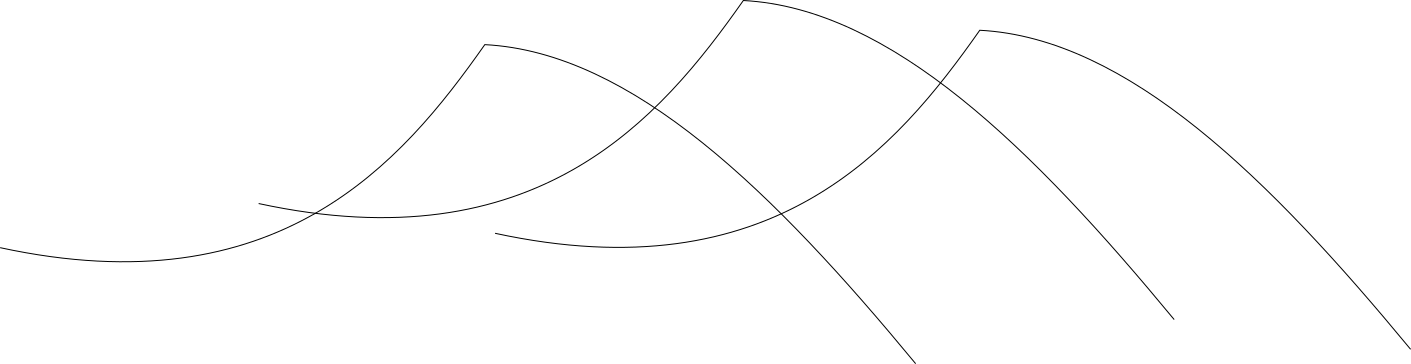
\includegraphics[width=0.63\textwidth]{example_graphic}
    \caption{Definitiv eine Vektor-Graphik. Weil die ja in Latex so angenehm sind. Will ich glatt als Hobby übernehmen so entspannt ist das, Vektor-Graphiken einzubinden.}
    \label{figure:test}
\end{wrapfigure}
Dies ist ein belangloser Fließtext. Dies ist ein belangloser Fließtext. Dies ist ein belangloser Fließtext. Dies ist ein belangloser Fließtext. Dies ist ein belangloser Fließtext. Dies ist ein belangloser Fließtext. Dies ist ein belangloser Fließtext. Dies ist ein belangloser Fließtext. 
Dies ist ein belangloser Fließtext. Dies ist ein belangloser Fließtext. Dies ist ein belangloser Fließtext. Dies ist ein belangloser Fließtext. 

\begin{wraptable}{l}{0.5\textwidth}
    \begin{longtable}{|l|l|l|}
        \hline
        Stadt   & Land     & Frucht  \\ \hline
        \endfirsthead
        %
        \endhead
        %
        Aachen  & Algerien & Apfel   \\ \hline
        Dresden & Dänemark & Dominik \\ \hline
    \end{longtable}
    \caption{Beispiel für eine Tabelle}
    \label{table:beispiel}
\end{wraptable}
Dies ist ein belangloser Fließtext. Dies ist ein belangloser Fließtext. Dies ist ein belangloser Fließtext. Dies ist ein belangloser Fließtext. Dies ist ein belangloser Fließtext. Dies ist ein belangloser Fließtext. Dies ist ein belangloser Fließtext. Dies ist ein belangloser Fließtext. 
Dies ist ein belangloser Fließtext. Dies ist ein belangloser Fließtext. Dies ist ein belangloser Fließtext. Dies ist ein belangloser Fließtext. 

\begin{wrapfigure}{r}{0.4\textwidth}
    \begin{equation}
        E=mc^2
    \end{equation}
    \caption{Eine sehr bekannte Formel}
    \label{equation:emc2}
\end{wrapfigure}
\Blindtext
\end{document}

\section{Analyse von Ergebnissen und Feedback}
\documentclass[crop=false]{standalone}
\usepackage{../imports}
\begin{document}
lorem ipsum

\end{document}

%
\chapter{Schluss}
\documentclass[crop=false]{standalone}
\usepackage{../imports}
\begin{document}
lorem ipsum

\end{document}

\section{Fazit}
\documentclass[crop=false]{standalone}
\usepackage{../imports}
\begin{document}
lorem ipsum

\end{document}

\section{Ausblick}
\documentclass[crop=false]{standalone}
\usepackage{../imports}
\begin{document}
lorem ipsum
\end{document}

\printbibliography[heading=bibnumbered]
\clearpage

\end{document}